% Agentic RAG với LangGraph 2
\begin{frame}{Agentic RAG với LangGraph}

\begin{figure}[H]
\centering
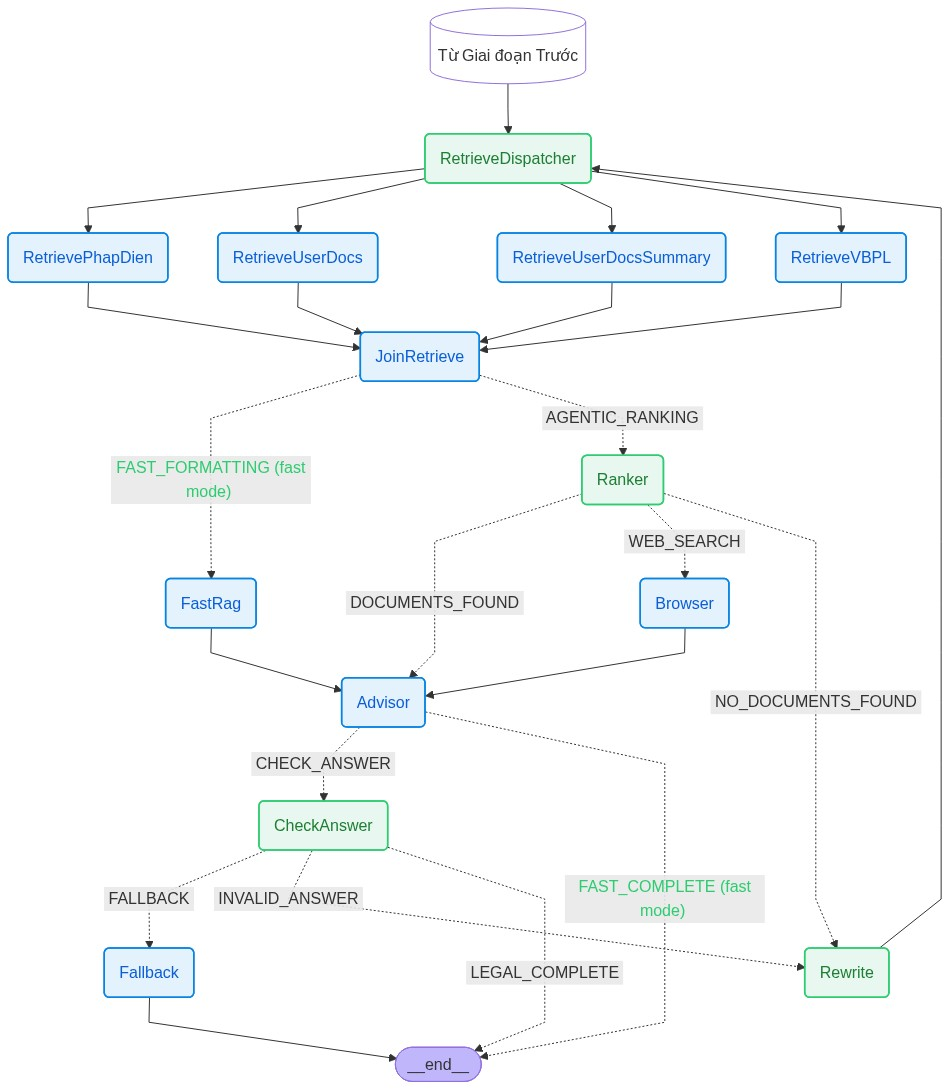
\includegraphics[width=\linewidth,height=0.740\textheight,keepaspectratio]{pictures/LangGraph/LangGraph2.png}
\caption{Sơ đồ LangGraph (Giai đoạn Truy xuất và Phản hồi)}
\end{figure}

\note{

Tiếp tục phần

Giai đoạn Truy xuất và Phản hồi

\hrule

Hệ thống thực hiện truy xuất
và lấy song song 4 nguồn dữ liệu:

tài liệu cá nhân +
tóm tắt tài liệu +
vbpl+
pháp điển

\hrule

Tiếp theo hệ thống

xếp hạng nguồn tài liệu

thử viết lại câu hỏi (nếu cần)

\hrule

Nếu nguồn tri thức không đủ

hệ thống lấy thông tin ở 2 trang web

thư viện pháp luật và luật việt nam

\hrule

Từ dữ liệu tổng hợp được
hệ thống đưa ra câu trả lời
và đánh giá xem có bị ảo giác hay không

}
\end{frame}

% tiếp tục phần giai đoạn truy xuất và phản hồi

% hệ thống thực hiện truy xuất
% và lấy song song 4 nguồn dữ liệu tài liệu cá nhân, tóm tắt tài liệu, văn bản pháp luật, pháp điển

% tiếp theo hệ thống xếp hạng nguồn tài liệu, thử viết lại câu hỏi (nếu cần). nếu nguồn tri thức không đủ hệ thống lấy thông tin ở 2 trang web thư viện pháp luật và luật việt nam

% từ dữ liệu tổng hợp được hệ thống đưa ra câu trả lời và đánh giá xem có bị ảo giác hay không
